\documentclass[]{article}

\usepackage[margin=1.0in]{geometry}
\usepackage{amsmath}
\usepackage{amsfonts}
\usepackage{amsthm}
\usepackage{graphicx}
\usepackage{amssymb}

\usepackage{mathtools}

\usepackage[
backend=bibtex,
style=alphabetic,
sorting=ynt
]{biblatex}
\addbibresource{refs}

\usepackage{hyperref}
\PassOptionsToPackage{hypernotes=false}{hyperref}

%opening
\title{Hejhal's Algorithm in $\mathbb{H}^3$}
\author{Alex Karlovitz}
\date{}

\begin{document}
	
	\maketitle

In this document, we describe Hejhal's algorithm as it applies to hyperbolic 3-space.
It is essentially the same as in 2-space; the differences occur only in the details of discrete groups acting on $\mathbb{H}^3$.
We begin with some background regarding hyperbolic 3-space, then we move on to Maass forms in this context.
After that, we will be ready to discuss the algorithm.

\section*{Preliminaries on $\mathbb{H}^3$}

By \textit{hyperbolic 3-space} (or $\mathbb{H}^3$), we mean the unique simply-connected Riemannian 3-manifold with constant sectional curvature -1.
There are various models of this space, but for now we will work with the upper half-space model.
Let the set $U^3$ consist of the subset of $\mathbb{R}^3$ with positive third component
$$
U^3 = \{ (x_1, x_2, y) \in \mathbb{R}^3 : y > 0 \}
$$
We endow $U^3$ with the metric
$$
ds^2 = \frac{dx_1^2 + dx_2^2 + dy^2}{y^2}
$$
It is well known that $(U^3, ds^2)$ is then isometric to $\mathbb{H}^3$.
Moreover, we note that $\mathbb{H}^3$ can be identified with the Hamiltonian quaternions whose $k$-term is 0.
That is, we take the subalgebra of
$$
\{ x_1 + x_2i + x_3j + x_4k : x_1, x_2, x_3, x_4 \in \mathbb{R}, i^2 = j^2 = k^2 = ijk = -1 \}
$$
whose elements have $x_3 > 0$ and $x_4 = 0$.
Replacing the name ``$x_3$'' with ``$y$,'' we evidently have the same set $U^3$.

\subsection*{M\"obius Transformations in 3-space}

Recall that $\text{SL}(2, \mathbb{R})$ acts on the upper half plane $\mathbb{H}^2$ via M\"obius transformations.
It is well known that these give all orientation-preserving isometries of hyperbolic 2-space.
In a similar fashion, $\text{Isom}^+(\mathbb{H}^3) \cong \text{PSL}(2, \mathbb{C})$.
Specifically, a given matrix acts on $\mathbb{H}^3$ via M\"obius transformations, where we interpret division as multiplication by the inverse in the quaternions:
$$
\begin{pmatrix}
\alpha & \beta \\
\gamma & \delta
\end{pmatrix}(z) =
(\alpha z + \beta)(\gamma z + \delta)^{-1}
$$
($z^{-1} = \bar{z}/|z|^2$).
If interested, one can find proofs of these facts online. (See, e.g., \href{http://www.maths.qmul.ac.uk/~sb/LTCCcourse/Holodyn2013notes_week3.pdf}{Holodyn 2013} for an outline).

To get a geometric feel for these transformations, it is instructive to consider the \textit{frame bundle} F$\mathbb{H}^3$ of hyperbolic space.
This is the set
$$
\text{F}\mathbb{H}^3 = \{ (z, v, w) \in U^3 \times \mathbb{R}^3 \times \mathbb{R}^3 : ||(v, w)||_z = 1, ~ v \perp w \}
$$
where the norm $||(\cdot, \cdot)||_z$ is derived from the hyperbolic metric.
(\textbf{TODO:} work out details for norm!).
One can show that $\text{PSL}(2, \mathbb{C})$ acts simply transitively on F$\mathbb{H}^3$, where the action is by
$$
g(z, v, w) = (g(z), \textbf{?}, \textbf{?}) ~~~~~ \text{Probably}~ (g(z), g'(z)v, g'(z)w)\text{? But need to think about derivative...}
$$
(\textbf{TODO:} work out details of action!)
Thus, we can identify $\text{PSL}(2, \mathbb{C})$ with F$\mathbb{H}^3$ by associating a matrix $g$ with the point $g(j, j, 1)$.
Intuitively, one thinks of $z$ as the base point in upper half-space, $v$ as a tangent vector pointing in the direction of a geodesic, and $w$ as a ``frame vector'' which is perpendicular to the tangent vector.
(Recall that geodesics in $\mathbb{H}^3$ are semicircles or vertical lines which are perpendicular to the $x_1x_2$-plane).

We now describe the geometry of the matrix action by describing how it moves the frame bundle.
First, recall the decomposition $\text{SL}(2, \mathbb{C}) = NAK$ where
$$
N = \left\{ 
\begin{pmatrix}
1 & u \\
~ & 1
\end{pmatrix} : u \in \mathbb{C}
\right\} ~~~~~
A = \left\{
\begin{pmatrix}
e^{t/2} & ~ \\
~ & e^{-t/2}
\end{pmatrix} : t \in \mathbb{R}
\right\} ~~~~~
K = M\text{SO}(2)M
$$
where $\text{SO}(2)$ is the special orthogonal group and
$$
M = \left\{
\begin{pmatrix}
e^{i\theta} & ~ \\
~ & e^{-i\theta}
\end{pmatrix} : \theta \in \mathbb{R}
\right\}
$$
Matrices from these three groups move the frame bundle in fairly simple ways.
\begin{itemize}
	\item A matrix in $N$ moves the point $(j, j, 1)$ to $(j + u, j, 1)$; that is, the base point is shifted by Re$(u)$ in the $x_1$ direction and by Im$(u)$ in the $x_2$ direction.
	In other words, $N$ moves points along the horosphere determined by the base point (horospheres in $\mathbb{H}^3$ are planes parallel to the $x_1x_2$-plane or spheres which are tangent to the $x_1x_2$-plane); the real part of $u$ determines the translation in the direction of the tangent vector, and the imaginary part determines the translation in the direction of the frame vector.
	\item Just as in hyperbolic 2-space, a matrix in $A$ moves points along geodesics at unit speed for time $t$.
	\item Matrices in $K$ fix the base point $j \in \mathbb{H}^3$ in $(j, j, 1)$ but can rotate the frame bundle to any position. Specifically, matrices in $M$ rotate the frame vector while leaving the tangent vector fixed, while matrices in SO(2) have the opposite effect.
\end{itemize}

\subsection*{The Action of Hyperbolic Elements}

We will be interested in subgroups $\Gamma \subseteq \text{PSL}(2, \mathbb{C})$ which act discontinuously on $\mathbb{H}^3$.
Such subgroups always contain \textit{loxodromic} elements (diagonalizable matrices with eigenvalues of norm not equal to $\pm1$).
In the special case where a loxodromic element has \textit{real} eigenvalues, we call the matrix \textit{hyperbolic}.
Now suppose $\Gamma$ contains a hyperbolic element $\gamma$, and let $g \in \text{SL}(2, \mathbb{C})$ diagonalize it.
Specifically, suppose
$$
g\gamma g^{-1} =
\begin{pmatrix}
\sqrt{\kappa} & ~ \\
~ & \sqrt{\kappa}^{-1}
\end{pmatrix}
$$
where $\kappa > 1$. Then there exists a fundamental domain for $g\Gamma g^{-1}/\mathbb{H}^3$ contained in
$$
F = \{ z \in \mathbb{H}^3 : 1 \leq ||z||_2 \leq \kappa \}
$$
since $g\gamma g^{-1}$ acts on the base points by scaling by $\kappa$.
When the group $\Gamma\backslash\mathbb{H}^3$ has infinite covolume, then such a fundamental domain must contain a positive-measure set in the $x_1x_2$-plane as part of its boundary.
We call these fundamental domains \textit{flare domains}, as the definition follows the same lines as those in $\mathbb{H}^2$.

\section*{Fourier Expansion in a Flare}

In the upper-half plane model of $\mathbb{H}^3$, the Laplacian is
$$
\Delta = -y^2\left( \frac{\partial^2}{\partial x_1^2} + \frac{\partial^2}{\partial x_2^2} + \frac{\partial^2}{\partial y^2} \right) + y\frac{\partial}{\partial y}
$$
To make use of the invariance under $z \mapsto \kappa z$ in a flare domain, we will utilize spherical coordinates.
Specifically, we write $(r, \theta, \varphi)$ for a point in $\mathbb{H}^3$, where $r$ is the (Euclidean) distance from the origin, $\theta$ is the angle of the projection onto the $x_1x_2$-plane measured counterclockwise from the positive $x_1$-axis, and $\varphi$ is the smaller angle measured off of the positive $y$-axis.
Note that since we are working with the upper-half plane model, $\varphi \in [0, \pi/2]$ with $\varphi = \pi/2$ indicating a point on the boundary.
In these coordinates, one can check that the Laplacian becomes
$$
\Delta = -\left(r^2\cos^2\varphi\frac{\partial^2}{\partial r^2} + \cot^2\varphi\frac{\partial^2}{\partial \theta^2} + \cos^2\varphi\frac{\partial^2}{\partial \varphi^2} + r\cos^2\varphi\frac{\partial}{\partial r} + \cot\varphi\frac{\partial}{\partial \varphi}\right)
$$

Next, suppose $f$ is a Maass form for $\Gamma\backslash\mathbb{H}^3$, where $\Gamma \subseteq \text{PSL}(2, \mathbb{C})$ contains the diagonal matrix whose action is $z \mapsto \kappa z$.
Then $f$ has a logarithmic Fourier expansion in $r$.
$$
f(r, \theta, \varphi) =
\sum_{n \in \mathbb{Z}}a_n(\theta, \varphi)e\left(n\frac{\log r}{\log\kappa}\right)
$$
Since $f$ is an eigenfunction of the Laplacian, we have $\Delta f = \lambda f$ for some $\lambda \in \mathbb{C}$.
This results in the following PDE for $a_n(\theta, \varphi)$
$$
\cot^2\varphi\frac{\partial^2}{d\theta^2}a_n(\theta, \varphi) + \cos^2\varphi\frac{\partial^2}{\partial\varphi^2}a_n(\theta, \varphi) + \cot\varphi\frac{\partial}{\partial\varphi}a_n(\theta, \varphi) + \left( \lambda - \frac{4\pi^2n^2}{\log^2\kappa}\cos^2\varphi \right)a_n(\theta, \varphi) = 0
$$
Let us fix $n$ for the moment and write $a_n(\theta, \varphi) = f(\theta)g(\varphi)$.
This separation of variables results in the two ODEs
$$
\begin{cases}
\frac{f''(\theta)}{f(\theta)} = C \\
\sin^2\varphi\frac{g''(\varphi)}{g(\varphi)} + \tan\varphi\frac{g'(\varphi)}{g(\varphi)} + \lambda\tan^2\varphi - \frac{4\pi^2n^2}{\log^2\kappa}\sin^2\varphi = C
\end{cases}
$$
where $C \in \mathbb{R}$ is some constant shared between the two equations.
Solving the equation in $\theta$, and using the fact that $a_n(\theta, \varphi)$ is invariant under $\theta \mapsto \theta + 2\pi$, one finds that
$$
f(\theta) = e^{im\theta}
$$
for some $m \in \mathbb{Z}$.
Note that this restricts the constant to $C = -m^2$.
\\

Alternatively, one could simply note that the invariance under $\theta \mapsto \theta + 2\pi$ implies $a_n(\theta, \varphi)$ has a Fourier expansion in $\theta$.
This lets us assume
$$
f(r, \theta, \varphi) = \sum_{m, n \in \mathbb{Z}}g_{m, n}(\varphi)e^{im\theta}e\left(n\frac{\log r}{\log\kappa}\right)
$$
Applying the differential equation $\Delta f + \lambda f = 0$, we can reduce to an ODE in $g_{m, n}(\theta)$ for each pair of $m, n \in \mathbb{Z}$.
Fixing $m$ and $n$ for the moment, we write $g = g_{m,n}$.
The ODE is then
\begin{equation}\label{gODE}
\sin^2\varphi g''(\varphi) + \tan\varphi g'(\varphi) + \left(m^2 + \lambda\tan^2\varphi - \frac{4\pi^2n^2}{\log^2\kappa}\sin^2\varphi\right)g(\varphi) = 0
\end{equation}
which is the same as we found using separation of variables above.
\\

In both methods, we are left trying to find a solution to (\ref{gODE}).
This can be converted to a hypergeometric differential equation as follows.
First, make the change of variables
$$
h(\cos^2\varphi) = \sin\varphi g(\varphi) ~~~ x = \cos^2\varphi
$$
Then equation (\ref{gODE}) reduces to
$$
4x^2(x - 1)^2h''(x) + \left( x^2 - \frac{4\pi^2n^2}{\log^2\kappa}x(1 - x) + m^2x + \lambda(1 - x) \right)h(x) = 0
$$
Some straightforward calculations show that $x = 0, 1, \infty$ are the three regular singular points of this differential equation.
Thus, the ODE has a hypergeometric function as a solution.
\\

We further note that since this is a second order homogeneous ODE, we expect a 2-dimensional vector space of solutions.
We reduce this to a 1-dimensional space by requiring the solution to be $L^2$ over a fundamental domain; since our fundamental domains contain flares, the infinite behavior will occur as $\varphi \rightarrow \pi/2$.
Recall that the Haar measure on hyperbolic space is $dx_1dx_2dy/y^3$.
In spherical coordinates, this is
$$
\frac{\sin\varphi drd\theta d\varphi}{r\cos^3\varphi}
$$
\textbf{TODO:} add Mathematica file to the github and make notes here on the formulas.

\section*{Example: Apollonian Circle Packing}

Recall that the Apollonian circle packing can be recognized as the orbit of circles in its ``cluster'' under reflections through circles in its ``cocluster'' (this is true for all ``crystallographic'' sphere packings; see \cite{kontorovich2017geometry} Theorem 31).
In Figure \ref{c_coc}, we show one realization of the cluster/cocluster decomposition for the Apollonian packing.
\begin{figure}[h]
	\centering
	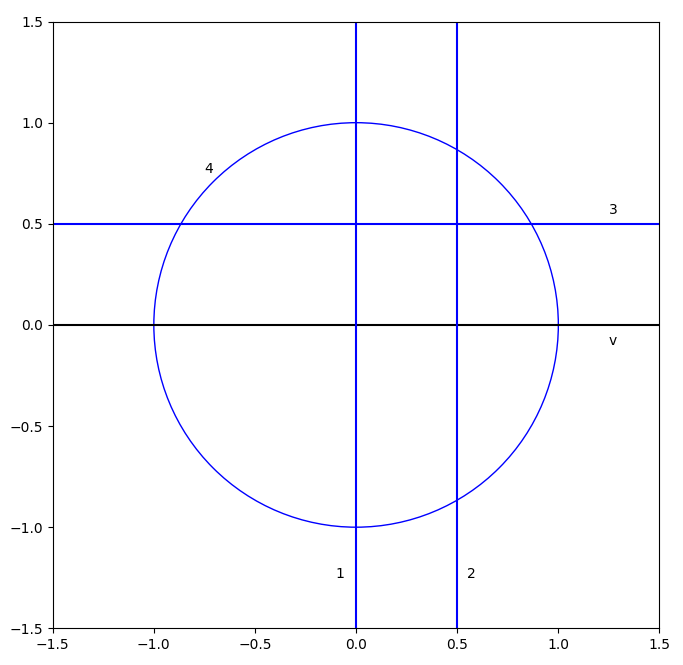
\includegraphics[width=0.5\linewidth]{cluster_cocluster.png}
	\caption{Cluster (black)/cocluster (blue) for the Apollonian packing}
	\label{c_coc}
\end{figure}
(Note that we think of lines as circles with infinite radius).
When the line $v$ is reflected through line 3, it gives a new line $w$; reflecting $w$ through circle 4 gives a circle of radius $1/2$ which is tangent to both $v$ and $w$.
In Figure \ref{orbit}, we see 21 circles in the orbit of $v$.
\begin{figure}[h]
	\centering
	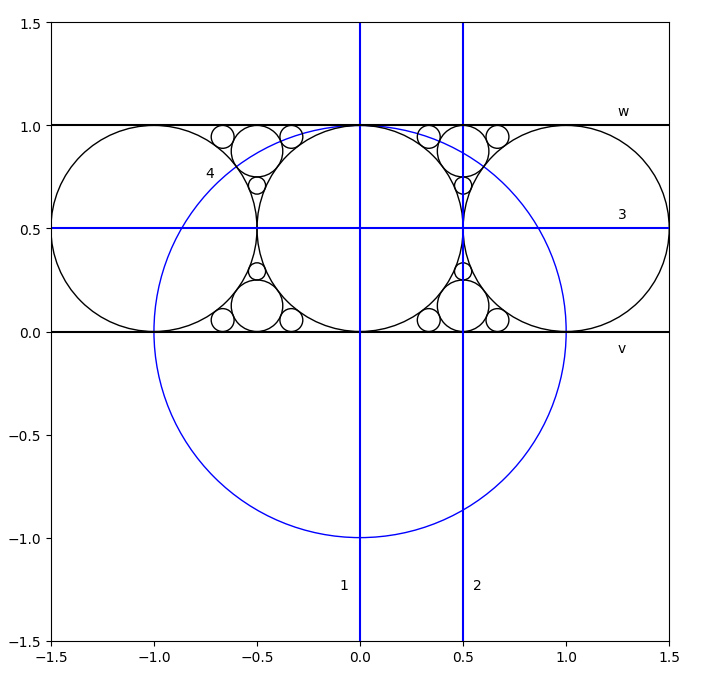
\includegraphics[width=0.5\linewidth]{some_circles.png}
	\caption{After various reflections through the cocluster (blue), we start to see the beginnings of an Apollonian circle packing (black)}
	\label{orbit}
\end{figure}

Another realization of the Apollonian circle packing is as the limit set of a reflection group in hyperbolic 3-space \cite{kontorovich2017geometry}.
Specifically, imagine drawing the cocluster in the $x_1x_2$-plane, then raising these to walls in the upper half-space model; that is, we raise circles to hemispheres and lines to vertical half-planes.
See Figure \ref{coc3d} for reference.
\begin{figure}[h]
	\centering
	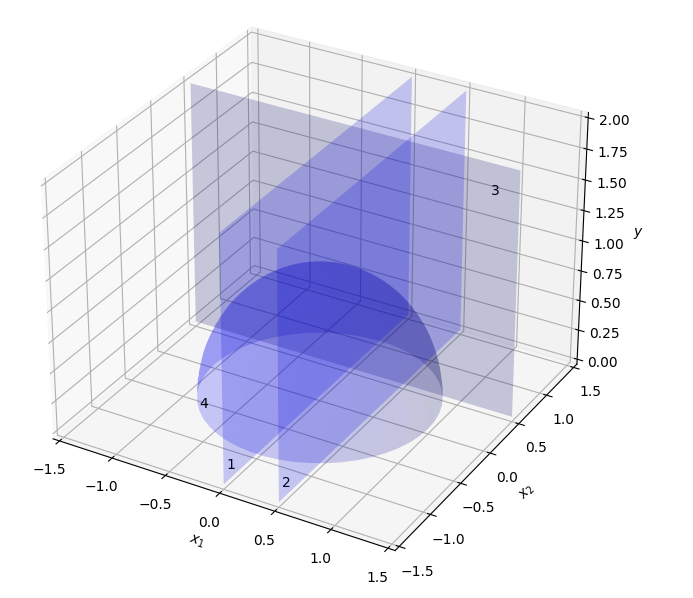
\includegraphics[width=0.5\linewidth]{cocluster_3D.png}
	\caption{The cocluster for the Apollonian packing raised into hyperbolic 3-space}
	\label{coc3d}
\end{figure}
\\ \\
\textbf{TODO:} add image to Figure \ref{coc3d} with orbits of lots of points. This should be experimental verification of the statement that the Apollonian packing is the limit set (proof in \cite{kontorovich2017geometry}).

\subsection*{Doubling the Reflection Group}

For use in Hejhal's algorithm, the group in question must consist of M\"obius transformations.
As in the 2-dimensional case, we achieve this by doubling our reflection group across one of the base reflections.
Let $R_i$ denote reflection through the $i^{th}$ wall for $i = 1, 2, 3, 4$, where the numbering is taken as in Figure \ref{coc3d}.
Then the reflection group $\Gamma$ can be written as
$$
\Gamma = \langle R_1, R_2, R_3, R_4 \rangle
$$
We will consider the group $\Gamma_0$ which is obtained by doubling $\Gamma$ across $R_1$.
$$
\Gamma_0 = \langle R_1R_2, R_1R_3, R_1R_4 \rangle
$$
In general, an even word in reflections through walls in $H^3$ is a M\"obius transformation; in this example, we can of course compute the actions directly.
One finds that
$$
R_1R_2(z) = z - 1 ~~~~~~~~ R_1R_3(z) = izi + i ~~~~~~~~ R_1R_4(z) = -\frac{1}{z}
$$
Thus, the corresponding matrices in $\text{SL}(2, \mathbb{C})$ are
$$
R_1R_2 \sim T^{-1} :=
\begin{pmatrix}
	1 & -1 \\
	0 & 1
\end{pmatrix} ~~~~~~~~
R_1R_3 \sim A :=
\begin{pmatrix}
	i & 1 \\
	0 & -i
\end{pmatrix} ~~~~~~~~
R_1R_4 \sim S :=
\begin{pmatrix}
	0 & -1 \\
	1 & 0
\end{pmatrix}
$$

Let us make a few immediate observations about the group $\Gamma_0 \cong \langle T, A, S \rangle$.
Clearly, $\Gamma_0 \leq \text{SL}(2, \mathbb{Z}[i])$.
Moreover, since $T$ and $S$ are the classic generators of $\text{SL}(2, \mathbb{Z})$, we see that $\text{SL}(2, \mathbb{Z}) \leq \Gamma_0$.
This fact can even be seen geometrically in Figure \ref{c_coc}; the area to the right of line 1, to the left of line 2, and outside circle 4 represents half of the usual fundamental domain for $\text{SL}(2, \mathbb{Z})$ in the upper half-plane.
Doubling across line 1 introduces the other half.
\\

To identify a fundamental domain $\mathcal{F}$ for $\Gamma_0$, we first note that the generator $T: z \mapsto z + 1$ allows us to map points into any width-1 interval in the $x_1$ coordinate.
We choose our fundamental domain with $-1/2 < x_1 < 1/2$; thus, $\mathcal{F}$ will be bounded by the half-plane 2 and the half-plane obtained by reflection 2 across 1.

Next, note that the generator $S : z \mapsto -1/z$ maps the unit sphere to itself while swapping its interior and exterior.
We will require points in $\mathcal{F}$ to have norm greater than 1; that is, hemisphere 4 provides another wall bounding our fundamental domain.
Finally, the generator $A: x_1 + ix_2 + jy \mapsto -x_1 + i(1 - x_2) + jy$ provides a bijection between points with $x_2 > 1$ and those with $x_2 < 1$.
So we take $\mathcal{F}$ to be on the side of half-plane 3 with $x_2 > 1$.

Thus, we can describe the fundamental domain $\mathcal{F}$ as the set
$$
\mathcal{F} = \left\{ z = x_1 + ix_2 + jy \in \mathbb{H}^3 : -\frac{1}{2} < x_1 < \frac{1}{2}, x_2 > 1, |z| > 1 \right\}
$$
In Figure \ref{doubled_coc_2d}, we show this fundamental domain in the $x_1x_2$-plane.
\begin{figure}[h]
	\centering
	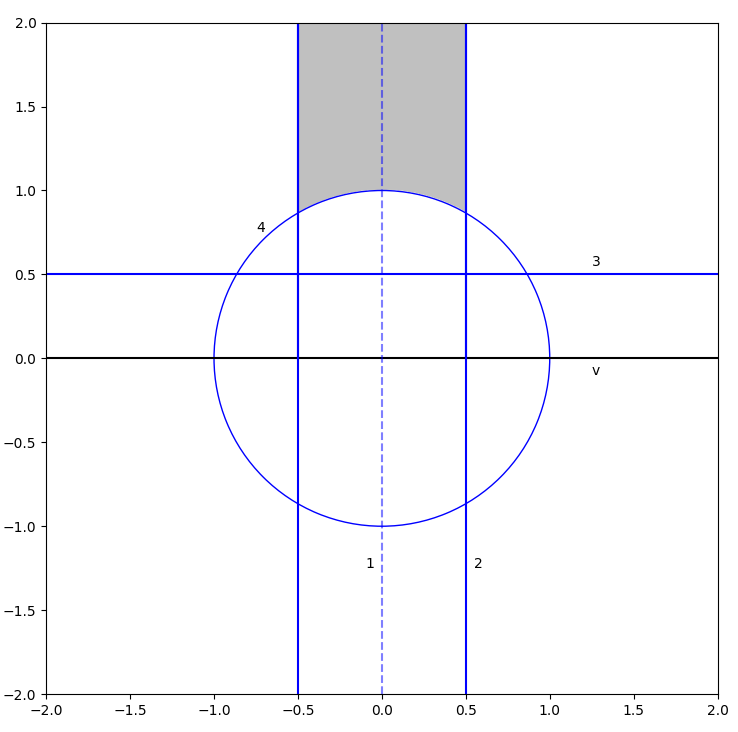
\includegraphics[width=0.5\linewidth]{doubledFD_in_plane.png}
	\caption{The cocluster for the Apollonian packing doubled across line 1; fundamental domain (intersected with $x_1x_2$-plane) shown in gray}
	\label{doubled_coc_2d}
\end{figure}
\\

We now consider a pullback algorithm to obtain the point in $\mathcal{F}$ corresponding to any given point in $\mathbb{H}^3$.
Here is pseudocode for the pullback; we assume the input is a point $z = x_1 + ix_2 + jy$ with $j > 0$.
\begin{verbatim}
if x2 < 1 :
    z = A(z)
    
repeat:
    # [[x]] := nearest integer to x
    z = T^(-[[x1]])(z)
    if |z| >= 1 :
        return z
    else :
        z = S(z)
\end{verbatim}
Note that $T$ does not change the $x_2$ coordinate.
Moreover, if a point $z = x_1 + ix_2 + jy$ has $x_2 >=1$ and $|z| < 1$, then applying $S$ to $z$ can only increase its $x_2$ component.
Thus, once we are in the ``repeat'' stage of the algorithm, we will never hit a point with $x_2 < 1$.
This is why we only need to apply $A$ at most once.
Inside the ``repeat'' loop, we are simply using $T$ to force $z$ into the strip $-1/2 \leq x_1 \leq 1/2$.
Then if $|z| < 1$, we apply $S$ to force the point outside of the unit sphere.
Note that within this loop, we are always increasing the $x_2$ component whenever we map by $S$.
Since $\Gamma$ acts discontinuously on $\mathbb{H}^3$, this loop must terminate in finitely many steps with a $z$ in the fundamental domain.
\\ \\
\textbf{TODO:} consider adding a 3D image of the fundamental domain (maybe bold the walls where they touch $\mathcal{F}$?)

\subsection*{Mapping to a Flare Domain}

To obtain a flare domain, we must identify a hyperbolic matrix in $\Gamma_0$.
Recalling that $\Gamma_0$ contains $\text{SL}(2, \mathbb{Z})$, we know that we have the matrix
$$
\gamma =
\begin{pmatrix}
	2 & 1 \\
	1 & 1
\end{pmatrix}
$$
One can check that $\gamma = T^2ST$, where $T: z \mapsto z + 1$ and $S: z \mapsto -1/z$ as defined above.
Recalling that $T = R_1R_2$ and $S = R_1R_4$, we could of course also write $\gamma$ in terms of the original reflections.

Next, one notes that $\gamma$ is diagonalized by $\gamma = P^{-1}DP$ where
$$
P =
\begin{pmatrix}
	\frac{-\sqrt{5}}{5} & \frac{5 + \sqrt{5}}{10} \\
	\frac{\sqrt{5}}{5} & \frac{5 - \sqrt{5}}{10}
\end{pmatrix} ~~~~~~~~
D =
\begin{pmatrix}
	\frac{3 - \sqrt{5}}{2} & 0 \\
	0 & \frac{3 + \sqrt{5}}{2}
\end{pmatrix}
$$
Since $\gamma \in \Gamma_0$, we have that $D \in P\Gamma_0P^{-1}$.
In particular, this implies $D^{-1} \in P\Gamma_0P^{-1}$, and $D^{-1}$ acts on $\mathbb{H}^3$ by scaling $z \mapsto \kappa z$ where
$$
\kappa = \frac{3 + \sqrt{5}}{3 - \sqrt{5}}
$$
This implies that $P\Gamma_0P^{-1}$ has a fundamental domain which is trapped between the unit hemisphere and the hemisphere centered at the origin with radius $\kappa$.
On the other hand, since $P\Gamma_0P^{-1}$ acts on $P\mathbb{H}^3$ in the same way that $\Gamma_0$ acts on $\mathbb{H}^3$, we note that one can obtain a fundamental domain for the conjugate group simply by applying $P$ to any fundamental domain for the original group.
In fact, as can be seen in Figure \textbf{ADD PIC}, the fundamental domain $P\mathcal{F}$ for $P\Gamma_0P^{-1}$ already constitutes a flare domain.

\pagebreak

\printbibliography

\end{document}